% vim:ft=tex
% rubber: module xelatex
\section{Our program}
The program is written in C++ using the Qt and OpenCV libraries, and
dependent on several other libraries including OpenSURF and IPOLdistortion.
The application consists of a Qt-based GUI that allows the user to load
images, select between various image processors, select parameters and
peruse the results of the processing by zooming and panning on the
output image. Furthermore, it is possible to select points of interest
(POIs) by double clicking on the image, which can be used to select
points for the calibration algorithm. The GUI also has a log output
window for textual output from the algorithms.

Each processor is implemented as a class that specifies which
parameters are available for this processor (the parameters can be set
by the user with the help of the QPropertySelect library), and does
the actual processing. The processing is done in a separate thread, to
keep the interface responsive, and make it possible for the user to
cancel a long-running processor.


% vim:ft=tex
% rubber: module xelatex
\subsection{Image segmentation}
\label{sec:segmentation}

We implemented two image segmentation algorithms: a simple thresholding algorithm, and a split and merge algorithm as described in the lecture slides. In both cases, the algorithm takes as input a greyscale image and outputs a segmented image. In the case of simple thresholding, the output image is divided into binary regions. In the case of the split and merge algorithm, the output image is divided into arbitrarily many regions, each one assigned a greyscale colour based on a rotating set of grey values.\\

The visible parameters and properties of the segmentation algorithms are:
\begin{itemize}
\item "Segmenting mode"; specifies the thresholding algorithm with either a global or adaptive threshold, or the split and merge algorithm.
\item "Dark background" (default false); specifies whether the input image has a dark or light background.
\item "Delta" (default 50); this is the parameter used for the uniformity predicate in the split and merge algorithm.
\item "Threshold"; this value updates with the calculated global or adapted threshold when the thresholding algorithm is being used.\\
\end{itemize}

The 'global threshold' form of the thresholding algorithm takes the mean of all the pixel intensities in the image, and sorts each pixel as belonging to the background or the foreground based on this threshold. The 'adaptive threshold' option begins with the global threshold, then iteratively adjusts it to be halfway between the means of the current background and foreground, adjusting what qualifies as a background or foreground pixel accordingly until the threshold converges. This simple algorithm has a user parameter which sets whether the background in the original image is light or dark; no attempt is made to automatically determine this property.

The split and merge algorithm is a form of contextual segmentation. The image begins as a single region. In each iteration of the "split" step, every region is quartered into subregions. This process continues until all regions are uniform. Then the "merge" step begins. In each iteration, adjacent regions are merged if the uniformity predicate would hold for the resulting superregion.

Typically, the behaviour of the "split" step would require input images with width and height powers of 2. This restriction is overcome by padding the edges with zero-intensity pixels to extend the image to the nearest power of 2. Regions made entirely of padding are then removed before the "merge" step. Regions made partly of padding are included in the "merge" step, but the resulting image is cropped back to its original parameters for the display.

In our implementation, the split and merge algorithm represents regions using the Region class. Unfortunately, in an attempt to be more efficient (by storing and processing fewer pixels), the Region class only stores the points of the regions' borders. The unforeseen downside of this is that the algorithm breaks down when non-convex regions exist. When the convexity assumption is broken, there are cases where regions that should have been merged escape the merging process, because certain pixels are included in checks that should not be. The result is that the segmentation process is less than perfect. The obvious solution to this implementation problem is to store all pixels which make up the region.

 In the "merge" step of the split and merge segmentation, regions are compared to each other rather naively (i.e. every region is compared to every other region). This slows the implementation considerably when there are more than a few hundred regions after the split step (which occurs for low values of the delta parameter and for extremely heterogeneous images). The solution would be to only consider merging regions that are neighbouring; this is unfortunately impossible to do efficiently with the current region representation. Regions are merged using 4-connectivity, in as far as the algorithm checks, for each pixel on the boundary of a region, in four directions to determine whether the region can be merged.

% vim:ft=tex
% rubber: module xelatex
\subsection{Face features extraction}

The first scale-invariant feature extraction algorithm was SIFT, described in \cite{SIFT}. SIFT is designed to be able to reliably detect features in altered (e.g. contrast-shifted, re-oriented or scaled) images. SIFT uses a database of training images with identified features to attempt to classify objects in new images based on their feature vectors. Image features are assumed to be the maxima and minima of the difference of Gaussians applied to the images. Outliers are discovered and removed by comparing each image feature with the model, verified by least squares.

The SURF extractor, described in \cite{SURF}, is an attempt to improve upon SIFT by speeding up computation without loss of computation quality or robustness. SURF achieves this improvement by convolving images with integral images, using a Hessian matrix-based detector, using a distribution-based descriptor, and simplifying to only 64 dimensions (see \cite{SURF}). An open-source implementation of this algorithm is OpenSURF, described in \cite{OpenSURF}. OpenCV also includes an implementation of the SURF algorithm. We use both these forms in our program, and add our own implementation of SURF. Our implementation is inspired by (and therefore structured similarly to) the OpenSURF implementation.

Our implementation uses the response layers and filter sizes from \cite{SURF}. This limits the range of possible values for the 'octaves' and 'intervals' parameters to (1-5) and (3-4) respectively. The OpenSURF implementation simply ignores the 'intervals' parameter in its calculations. The process of estimating the determinant of the Hessian matrix from the filter response values requires a weight for the $D_{xy}$ direction. We follow \cite{SURF} in setting this weight to $0.9$.

The three implementations (ours, OpenCV and OpenSURF) use different threshold values for the algorithm. It appears (with the caveat that it is difficult to tell because the code is quite convoluted) that OpenCV does not area-normalise the values. This is likely the reason for the discrepancy between our implementation and that of OpenCV. OpenSURF represents greyscale values as floating point values between 0 and 1, whereas we represent them as int values between 0 and 255, which should account for the second discrepancy between threshold values.

The interpolation between points to get subpixel accuracy for interest points follows the method in \cite{inv-features}; this essentially amounts to solving a linear system using pixel differences as approximations for the derivatives. In \cite{SURF}, it is implied that this process should be used to iteratively interpolate keypoint locations, and discard those that do not converge. However, both OpenCV and OpenSURF appear to simply use the interpolation deltas to discard keypoints that interpolate to a different point, rather than attempting to iterate towards convergence. Our program follows these implementations in abandoning the iterative paradigm. We found, though, that using interpolation for subpixel accuracy \emph{at all} appears to make our implementation 'worse' (in that its results diverge from that of the OpenCV and OpenSURF implementations). Why this should be the case is unclear.

\paragraph{Experimental process.}
To test the capability of our own algorithm implementation, we ran it on six images of human faces. Credit is given to the Massachusetts Institute of Technology and to the Center for Biological and Computational Learning for providing the database of facial images; see \cite{database}. The forward-facing images subset of the MIT-CBCL database was used. We first manually extracted features from the original images, identifying 10 interest points (eye centres, eye corners, mouth corners, mouth centre, tip of nose) in each case. 
For each face, we tested 40 threshold values (from 1 to 196, differing by 5 in each case). We noted the number of interest points correctly identified as features (counting a hit within 15 pixels of the manually identified feature as a success). As well as these true positives, we also noted the number of false negatives (interest points not identified as features) and false positives (other points incorrectly identified as features).





% vim:ft=tex
% rubber: module xelatex
\subsection{Camera calibration}
\label{sec:calibration}
For the camera calibration part of the application, we have
implemented the calibration algorithm from \cite{TSAI}, which is a
classical and often cited calibration method. The article encompasses
several different methods of calibration; we are implementing the
method that the article describes as "the monoview non-coplanar
case''. That is, the calibration is performed from a single image
of a calibration object that has calibration points in several (world)
planes.

Our calibration object can be seen in figure~\ref{fig:calib-object}.
It consists of two adjacent faces of a cube, each of which has a
number of circular calibration points. The left face has 35 points,
and the right face 28. The distance between point centres is 1,5
inches. The world coordinate system is chosen to be a right-handed
coordinate system, centred at the bottom corned of the cube, so the
left face corresponds to the YZ plane, and the right face corresponds
to the XZ plane.

\begin{figure}[hb]
  \centering
  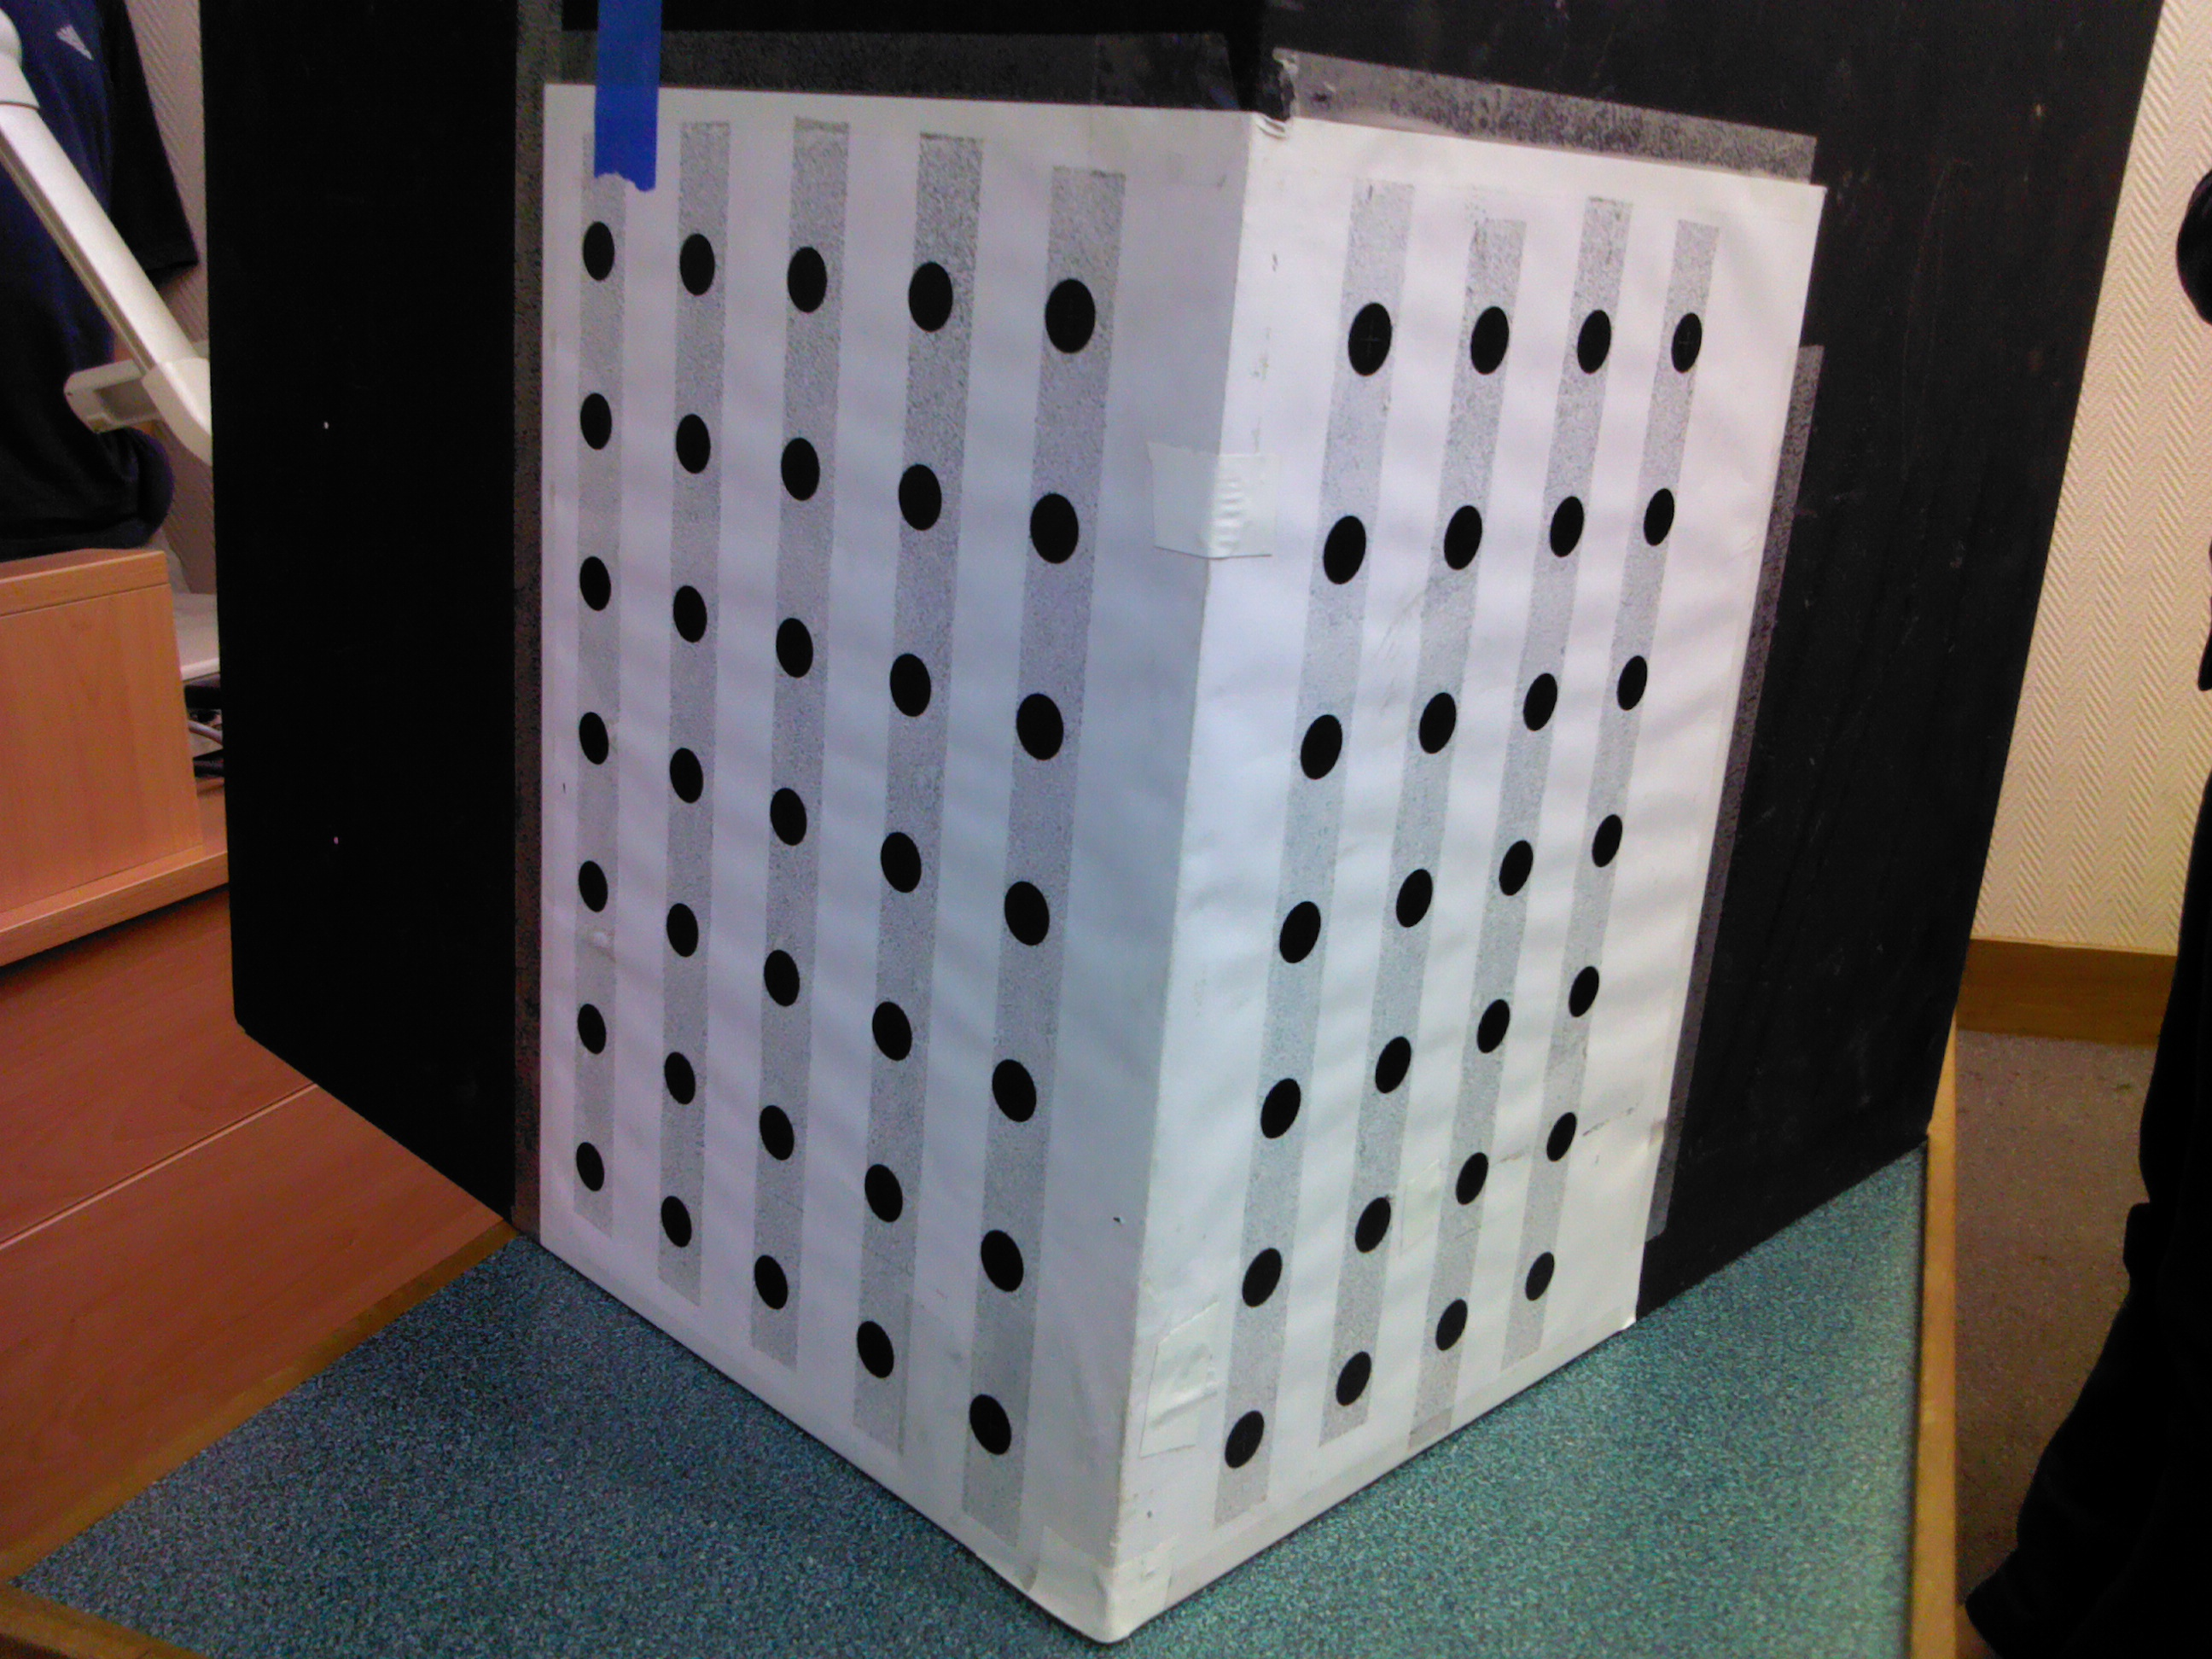
\includegraphics[width=0.7\textwidth]{figures/calibration-object}
  \caption[Calibration object]{Calibration object. The left face has
    35 calibration points (the centres of the circles), and the right
    face has 28. The distance between point centres is 1,5 inches. The
    world coordinate system is chosen to be a right-handed coordinate
    system, centred at the bottom corned of the cube, so the left face
    corresponds to the YZ plane, and the right face corresponds to the
    XZ plane.}
  \label{fig:calib-object}
\end{figure}

\subsubsection{Implementation notes}
The implementation overall follows the procedure laid out in
\cite{TSAI}. However, a few notes on the implementation are
appropriate:

\paragraph{Implemented parts of the algorithm.}
As mentioned, we implement the calibration method that Tsai refers to
as ``the monoview non-coplanar case''. The calibration function derives
the transformation matrix, composed of the rotation matrix, $R$ and
the translation matrix $T$, find the scale factor $s_x$, and the
intrinsic camera values $f$ (focal length) and $\kappa$ (radial
distortion parameter). The radial distortion is calculated as far as
$\kappa_1$. The literature suggests that this is sufficient for
reasonably high accuracy using cameras without significant lens
distortion \cite{algebraic-distortion}.

\paragraph{Mapping of image coordinates to world coordinates.}
The world coordinates of the points are measured manually, in units of
inches. These are given as input to the program in the form of a
space-separated text file. The image coordinate points are found by
first running the SURF feature point extraction algorithm described in
section~\ref{sec:features} on the input image, with a relatively high
threshold value (500). The feature points detected using this
algorithm are shown to the user on a binary image (obtained using
adaptive thresholding -- see the description of the segmentation
algorithms in section~\ref{sec:segmentation}), who then has the option
of removing and adding points.

These user-corrected points are fed to the second stage of the
calibration algorithm. This stage assumes that there are exactly 63
points selected on the image, and furthermore takes as input exactly
63 3D points (corresponding to the 63 circles on the calibration
object). The image points are first corrected to be closer to the
centre of the circle. This is done by flood filling the binary image
from each point with a threshold of 0 (i.e. finding all pixels of the
same colour as the point), and taking the average x and y values from
this region. This means that the user does not have to select points
that are exactly at the centre of the calibration region, but can
click anywhere within it.

Following this correction, the image points are mapped to the real
world coordinate points. This is done by a brute-force algorithm
relying on the fact that
\begin{inparaenum}[(a)]
  \item the right and left faces are entirely disjoint in the
    horizontal direction, i.e. no points on the right face have
    x-coordinates lower than any points on the left face, and
  \item the top and bottom outermost points in each face are the
    points closest to the respective image corners on that side of the
    image.
\end{inparaenum}
This algorithm does impose some limitations on the possible viewing
angles of the calibration object. For example, if the image is rotated
by enough to make the faces overlap in the horizontal direction, the
first assumption breaks down and the image point to world point
mapping fails.

\paragraph{Back-projection.}
To test the error ratio of the calibration, we reverse the direction
of projection, by projecting the rays from the camera through the
image coordinate points onto the corresponding face planes in world
coordinates (taking into account the (reversed) calibration
parameters). This allows us to measure the distance between these
derived world coordinates and the known ones as an error radius.

\paragraph{Implementation problems.}
We have encountered a few problems in our implementation. Primarily,
it was not completely obvious to us that, in going from the coplanar
to the non-coplanar cases, equation (15) in \cite{TSAI} has to be
re-derived from the earlier equation (8b), because the it is no longer
true that $z_w=0$. Also, it proved tricky to get the back-projection
working correctly.

\subsection{Experimental results}
For testing the calibration, we have run the program on four different
pictures of the calibration object, taken with two different cameras.
In this section, we go thnrough the results, first by doing some sanity
checking on the values from observations of the environment, and then
by looking at the errors from the back-projection estimates.

\begin{table}[htb]
  \centering
  \begin{tabular}{c c c c c c}
    \toprule
    \multicolumn{3}{c}{\textbf{Rotation}} & \multicolumn{3}{c}{\textbf{Translation}}\\
    \midrule
    \multicolumn{3}{c}{$R=\begin{bmatrix}0.69 & -0.72 & 0.08\\
    0.14 & 0.25 & 0.96\\
    -0.70 & -0.65 & 0.28\end{bmatrix}$} &
    \multicolumn{3}{c}{$T=\begin{bmatrix}0.00\\-6.76\\-16.80\end{bmatrix}$} \\
    \midrule
    \multicolumn{2}{c}{\textbf{Scaling}} &
    \multicolumn{2}{c}{\textbf{Focal length}} &
    \multicolumn{2}{c}{\textbf{Distortion}}\\
    \midrule
    \multicolumn{2}{c}{$s_x =0.998$} &
    \multicolumn{2}{c}{$f=-2424.61$} &
    \multicolumn{2}{c}{$\kappa_1=-1.76 \cdot 10^{-8}$}\\
    \bottomrule
  \end{tabular}
  \caption[Calibration results]{Calibration results. This is the
    results of calibration for the first image (labelled 160019 in
    figure~\ref{fig:calib-errors}).}
  \label{tbl:calib-results}
\end{table}

One of the results of the calibration can be seen in
table~\ref{tbl:calib-results}. Looking at the translation vector,
according to the calibration, the corner of the calibration object is
just under 17 inches in front of the camera (or camera plane) and just
under 7 inches below it. These figures are roughly consistent with the
distance from which the picture is taken, so the calibration does not
appear to be completely off.

Furthermore, in table~\ref{tbl:focal-lengths} is a comparison
between the focal length results for the four images. From this, it is
apparent that images taken with the same camera have similar focal
lengths, and the focal lengths of images taken with different cameras
are quite different. These two sanity tests together suggest that the
results of the calibration are not completely off.

\begin{table}[h]
  \centering
  \begin{tabular}{c c}
    \toprule
    \textbf{Image} & \textbf{Focal length}\\
    \midrule
    160019 & -2424.61\\
    160027 & -2412.75\\
    0025 & -4887.01\\
    0026 & -4701.72\\
    \bottomrule
  \end{tabular}
  \caption[Focal length values for the test images]{Focal length
    values for the test images. The images are taken pairwise with two
    different cameras; this is reflected in the focal length values,
    in that images taken with the same camera have very similar focal
    lengths, and there is a large variation between the two cameras.}
  \label{tbl:focal-lengths}
\end{table}

To test the size of error in the calibration values, we have
implemented a back-projection test, as described in the previous
section. From this, we have obtained mean radii of error, i.e. the
distances from the back-projected points to the known locations of the
interest points. These are summarised in
figure~\ref{fig:calib-errors}. The mean errors are roughly four times
the errors Tsai reports in his paper (mean error $0.7$ mm $\simeq0.02$
inches). The fifth column of the figure shows the mean error for one
of the images, using only the eight centre-most calibration points.
This error is not much different from when all 63 points are used, and
we suspect at least not significantly\footnote{We have unfortunately
  misplaced the data that would allow us to confirm this with a proper
  statistical model.}.

\begin{figure}[htb]
  \centering
  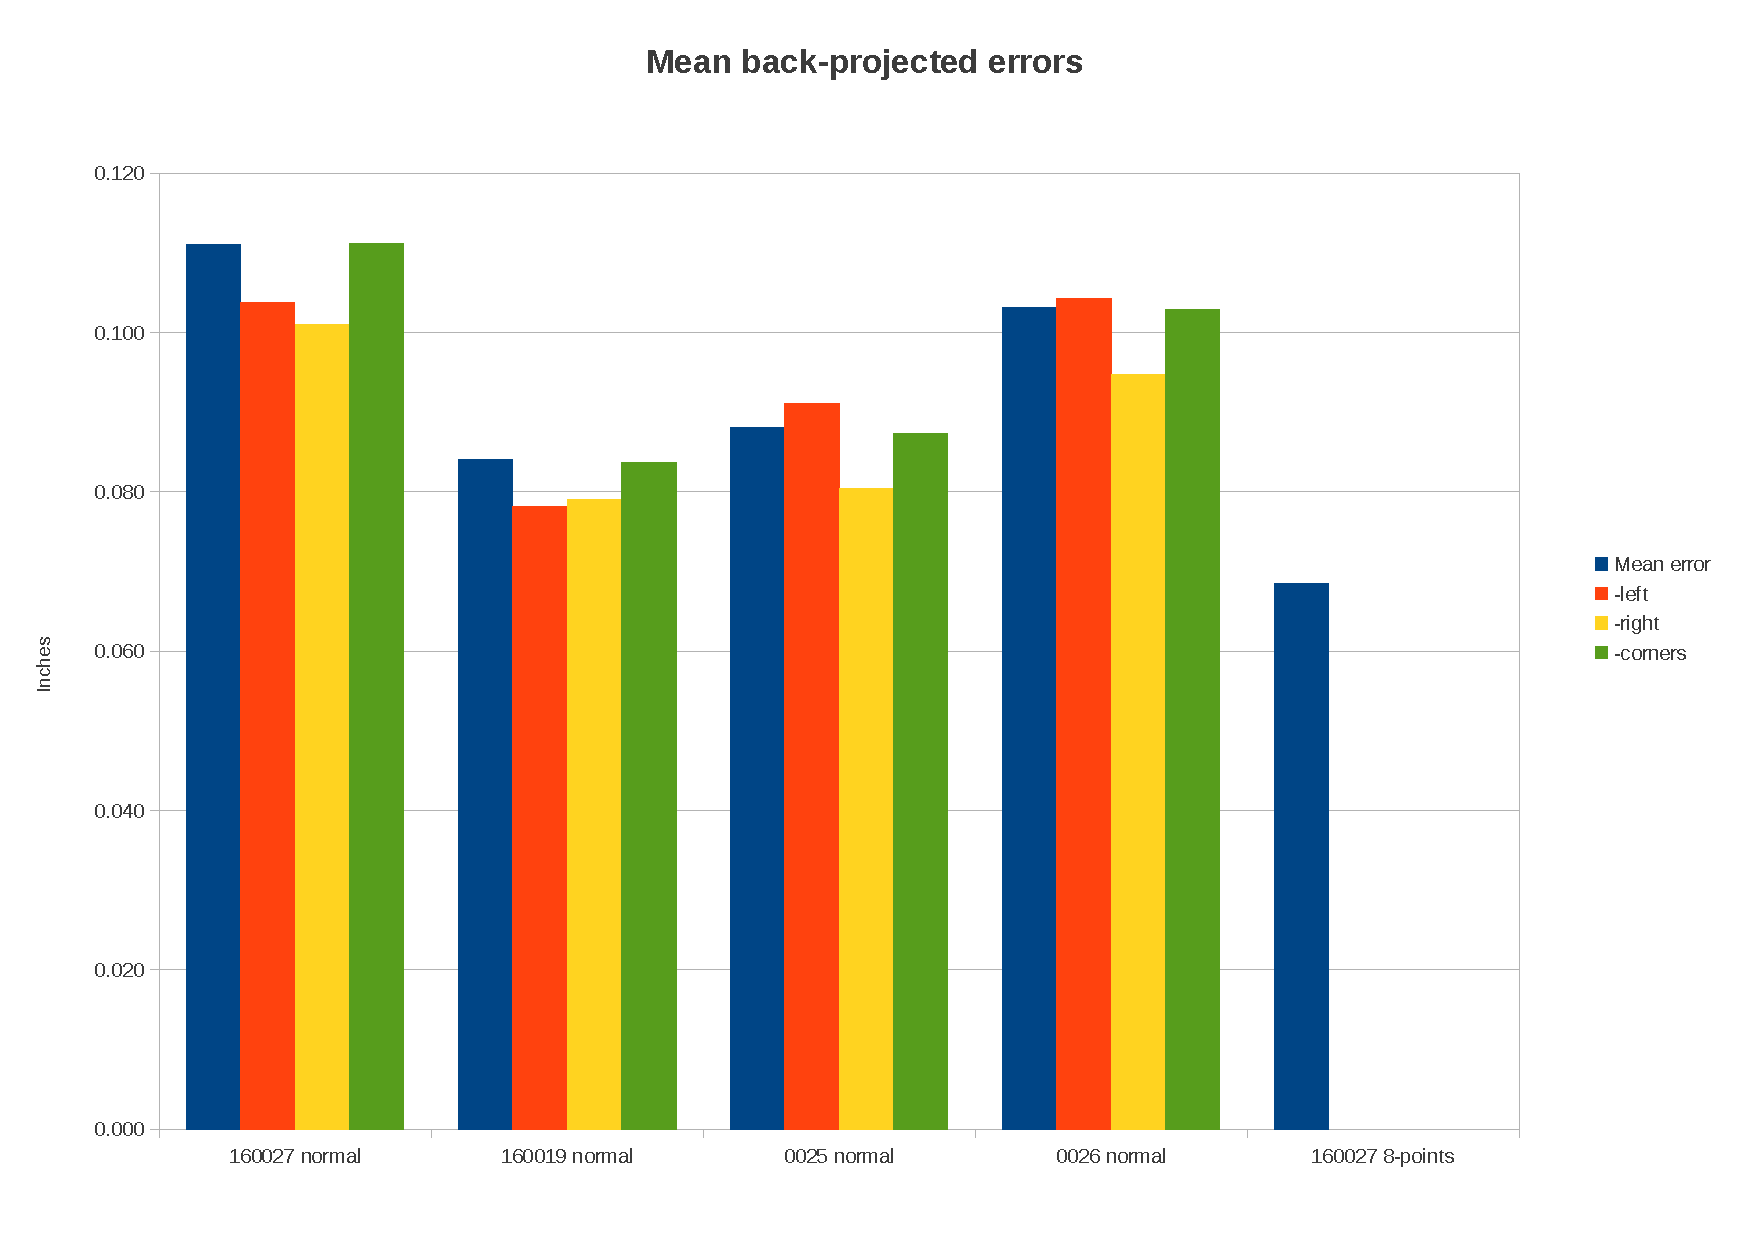
\includegraphics[width=0.7\textwidth]{figures/calibration-means}
  \caption[Mean calibration errors]{Mean calibration errors for all
    calibration points. Each set of bars is from a different image of
    the same calibration object. The images are taken with two
    different cameras, two with each camera. The lone bar on the right
    is the mean error calculated from the first image, but with only
    the 8 centre-most calibration points.}
  \label{fig:calib-errors}
\end{figure}



%Calibration experiments:\\
%
%-> On eight images (2 low grade, 2 high grade, 2 low grade distorted,
%2 high grade distorted)...\\
%
%-> Compare backprojection accuracy... mean, variance, worst hit, best
%hit, breakdown into (x,y,z) \\
%
%-> Compare kappa calculated (should be higher with lens distortion...
%but using actual fisheye distortion may be so high that the polynomial
%kappa model is unsuitable for it, as \cite{straightlines} (I believe
%ot was) suggests can happen).\\
%
%-> Subjectively, look at the resulting translation and rotation
%matrices and consider what they mean, as well as the sx and
%focalLength.\\
%

% vim:ft=tex
% rubber: module xelatex

\subsection{Distortion removal}

% http://dl.acm.org/citation.cfm?id=1924387
% http://scien.stanford.edu/pages/labsite/2007/psych221/projects/07/geometric_distortion/project.htm
% http://www.embedded-vision.com/industry-analysis/technical-articles/2011/05/14/lens-distortion-correction

% "Straight lines ought to be straight" - \cite{straightlines} .\\
% "Applying and removing lens distortion in post production" - \cite{postproduction} .\\

We investigated forms of distortion removal independent of camera calibration. One particularly useful and simple open-source ANSI C library we discovered was provided by the authors of \cite{algebraic-distortion}. Herein we shall refer to this IPOL library and the algorithm it describes as IPOLdistortion. This implementation estimates the lens distortion parameters of a camera (or image) based on the rectification of lines in the images, as described in e.g. \cite{straightlines}, but with some innovations.

\cite{algebraic-distortion} find the lens distortion parameters by minimizing a 4 total-degree polynomial in several variables. The mathematical theory behind their implementation (for which see 

?????

) leads the authors to only consider kappa-0, kappa-2 and kappa-4. See the paper cited for a full explanation. The algorithm functions by setting the first distortion parameter to 1 (to avoid the trivial solution kappa-0 = 0), and then minimising a distortion error measure function in the form of an energy function of the authors' design. This function is a real-valued polynomial in the variable kappa. To minimise the function, IPOLdistortion finds the solutions to the algebraic system of equations generated by its gradient. The implementation also introduces a "zoom factor" minimising the distance between distorted and corrected points, in order to to create corrected points as close as possible to the distorted ones \cite{algebraic-distortion}.

\subsubsection{Implementation notes}

The IPOLdistort library requires that users manually select points on the straight line for the algorithm to work on. This is both an arduous process and susceptible to human error. Furthermore, \cite{algebraic-distortion} state that for the maximum efficacy, as many straight lines as possible should be used. Therefore in our implementation, we combine the distortion correcting functionality of IPOLdistort with the line extraction functionality of OpenCV. 

We use OpenCV to automatically extract detected corner points from a (distorted) chessboard image. From these corner points, and our knowledge of the chessboard dimensionality (number of squares per side), we can reconstruct segments which "should" be straight lines in the image. The algorithm we use for this is relatively naive, relying on the fact that OpenCV returns corners in a fixed order. The algorithm is likely to fail if this list is out of order for some reason, or if a subset of points is not returned. For the best performance, the algorithm should take multiple vertical and horizontal lines as input. We therefore provide it with all the horizontal lines returned by the OpenCV code, as well as two vertical lines reconstructed from these.

The actual distortion removal functionality provided by IPOLdistortion consists of first modelling the distortion and then correcting the image based on that model.



blah blah
This is done using an open-source library which uses an optimizer to determine the undistorted coefficients by minimizing the error between the radial distortion model and the image data.
5. Note that this usage of the algorithm only works within certain constraints: only on relatively 'clean' images of [distorted] chessboards (due to opencv), and only on uncompressed .tif images (due to the IPOLdistort library).\\
5.a) (We our work to be an extension of the functionality of IPOLdistortion, which requires the user to input line segments by hand. Further work would obviously extend the functionality to cover non-chessboard images.)\\
6. SEE the IPOLdistortion readme for a good (simple) explanation; it is based on \cite{algebraic-distortion}.\\\\



\subsubsection{Experimental process.}

\paragraph{Experimental parameters.}
To test our program, 

Distortion removal experiments:\\
-> We created a suite of 22 different 8x8 chessboard images. These included variations on rotation, position, barrel and pincushion distortion, other forms of distortion, and noise.\\
-> We compare calculated  lens distortion parameters (kappas) on different chessboard types.\\
-> We also checked that chessboards of varying dimensionality can be used. This is successful for chessboards with side lengths at minimum 4, and up to length 16 or more (assuming the size of each chessboard square remains the same).
-> Finally, comparison with camera calibration results: we generated lists of lines for each face of three images, 0027, 0027 with barrel distortion, and 0027 with pincushion distortion. We generated straight lines from the image calibration points, which obviously ought to lie on straight lines. For each case, we used all horizontal lines and the two outer vertical lines from each face. We ran distortion removal on these, and compared the kappa-0, kappa-2 and kappa-4 output of the distortion algorithm to the kappa-1 found by calibration.\\

\paragraph{Experimental results.}
(INSERT CHARTS HERE)

Note that \cite{algebraic-distortion} state, "we will always take the center of the image as distortion center".





